\chapter{Computação e Síntese de Voz}
	
	\subsection{Modelo Mono-Massa}
	
	Os modelos de uma massa são os mais simples para se representar as pregas vocais,com essa única massa representando toda a estrutura das pregas vocais. Como é representado por uma massa somente, o grau de liberdade neste sistema é 1, ou seja, o deslocamento é dado somente em uma direção~\cite{SpeechComunication}. Conforme foi citado no Capítulo 2, para um modelo viscoelástico das pregas vocais apresentar auto-oscilação, energia deve ser periodicamente adicionada ao sistema de modo que supere as fricções internas do tecido laríngeo. Tal energia é acrescida ao sistema por uma carga externa quando a mesma está em fase com a velocidade de vibração das pregas vocais.
	
	A modificação na pressão aerodinâmica devido às mudanças de orientação convergente divergente da glote é o mecanismo primário pelo qual o supracitado ocorre fisiologicamente. Por definição, os sistemas mono-massa não podem desenvolver por si só a variação(no tempo) glotal necessária para que as pressões supraglotal e glotal sejam carregadas assimetricamente, permitindo que o efeito de Bernoulli aja em reconhecimento à abertura e fechamento da glote. Para que isso ocorra neste sistema, deve haver uma interação da glote com um tubo acústico supraglotal ou subglotal ~\citealp{IngoTitze}.
	
	Considere agora o sistema representando cada prega vocal, cujos componentes são uma massa m, uma constante de rigidez k e uma constante de amortecimento b. A constante de amortecimento representa a viscosidade do tecido, ou seja, atua como um absorvedor de energia. A constante k representa as propriedades elásticas do tecido ao passo que m é a massa do tecido em movimento, Figura~\ref{fig:monoMassa}.
	
	
	\begin{figure}
		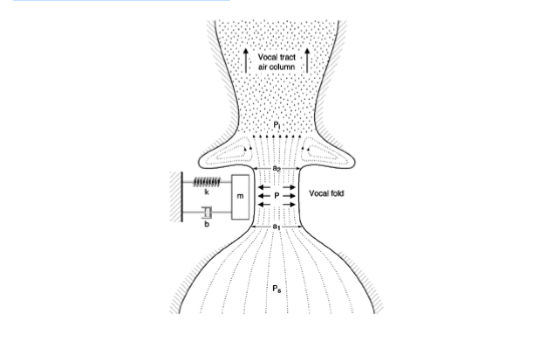
\includegraphics{monoMassa}
		\caption{Modelo Mono-Massa~\cite{IngoTitze}}
		\label{fig:monoMassa}
	\end{figure}
	
	A pressão P na glote atua perpendicular à superfície do tecido. Se esta pressão se alterar de acordo com a direção da velocidade, então energia será transmitida ao tecido pelo fluido, e esta pode superar a energia perdida com a viscosidade do tecido. Entretanto, como essa pressão pode ser diferente ou as simétrica no caminho de volta do que foi ao sair? Ou seja, como a pressão pode ser alterada e consequentemente acompanhar e influenciar a abertura e o fechamento da glote?
	
	Titze derivou uma expressão para a pressão intraglotal na superfície das pregas vocais[26] e forneceu uma versão simplificada dessa expressão para o modelo em questão~\cite{IngoTitze}, conforme mostra a equação~\ref{eq:7}

	
	\begin{equation}
		\centering
		\[
			P = ( 1 - \frac{a_2}{a_1}) * (P_s - P_i) + P_i
		\]
		\label{eq:7}
	\end{equation}
	
	Onde $a_1$ e $a_2$ são as áreas de entrada e saída da glote respectivamente, Ps é a pressão subglótica e Pi é a pressão exercida sobre o trato vocal, chamada de pressão de input. O primeiro termo da equação é um fator geométrico que descreve o formato da glote. O segundo termo, a diferença de pressões, descreve a pressão transglotal, ou seja, aquela que percorre a glote. Para o modelo mono-massa, temos que a1 = a2 o que faz com que a pressão intraglotal seja simplesmente equivalente à pressão supraglotal. 
	
	A relação resultante de que a pressão condutora P é igual à pressão supraglotal sugere que algo deve acontecer acima da glote para que essa pressão seja alterada durante o ciclo glotal. O elemento chave aqui é a inércia do ar no trato vocal. A lentidão em resposta da coluna de ar acima das pregas vocais causa uma outra condição de superação que auxilia na vibração, isto porque quando a glote está abrindo e o fluxo de ar aumentando, a coluna de ar está sendo acelerada pelo fluxo glotal. Isto cria uma pressão positiva Pi na entrada do trato vocal, fazendo com que as pregas vocais se separem. Essa pressão positiva gera também um aumento no ímpeto(ou na quantidade de movimento) da coluna de ar. Quando a glote fecha, o ímpeto da coluna de ar continua e o fluxo na glote não se sustenta com o fluxo da coluna de ar, gerando uma pressão negativa(sucção) acima das pregas vocais auxiliando no fechamento das pregas vocais. Portanto, Pi conduz as pregas vocais em sincronia com seu movimento natural. 
	
	Essa explicação é muito similar ao efeito de Bernoulli em ação, entretanto, um termo adicional muito importante está envolvido: o atraso na resposta à pressão da coluna de ar no trato vocal. 
	
	Dessa maneira, fica claro que em decorrência do grau de liberdade do modelo mono massa, não há como este modelo reproduzir uma movimentação ondular das pregas vocais, o que auxiliaria na criação e manutenção da auto-oscilação. Em decorrência disso, o trato vocal atua suprindo esta falta de modo que o mesmo possibilita a alteração nas pressões durante as fases de movimento das pregas vocais o que induz uma auto-oscilação no sistema mono-massa, conforme explicado.
	
	
	\subsection{Modelo Computacional para Representação do Trato Vocal}
	
	Para a representação do trato vocal, Fraj ~\cite{JeanFrancis}, Titze ~\cite{IngoTitze} descrevem um modelo físico, onde o trato vocal é representado como uma concatenação de pequenos tubos cilíndricos de tamanhos variados e consequentemente de áreas diferentes. As condições de continuidade da pressão acústica e da velocidade do fluido em cada junção de tubos permite o mapeamento das ondas acústicas depressão e de velocidade de entrada com as de saída. Aplicando isso interativamente, obtêm-se a simulação da propagação da onda no trato vocal. Levando em consideração que o tempo de propagação em um duto equivale à uma amostra no sistema, é possível aproximar o tamanho necessário dos tubos cilíndricos de acordo com a frequência da amostra e a velocidade do som. 
	
	Existem dois modelos para a representação do trato vocal como um concatenação de tubos cilíndricos. O primeiro, foco deste trabalho, é chamado de modelo de reflexão de onda ~\cite{BradhStory}~\cite{JeanFrancis}. O segundo, caso haja interesse em pesquisa, é chamado de modelo linha de transmissão e pode ser também encontrado no livro de Titze~\cite{IngoTitze}.
	
	\subsection{Modelo de Reflexão}
	
	Este modelo tem seus fundamentos na reflexão das ondas sonoras no trato vocal, conforme citado no Capítulo 2. Enquanto a glote produz uma onda acústica com muitas frequências, o trato vocal amplifica um subconjunto dessas frequências para radiar pela boca. O filtro desses subconjuntos está diretamente ligado às características de ressonância e reflexão do trato vocal, e é isto que este modelo busca implementar. 
	
	
	\subsubsection{Impedância Acústica em um Tubo}
	
	Se a velocidade média de uma partícula for multiplicada pela área transversal do tubo, um fluxo médio pode ser obtido. Esse fluxo médio é conservado quando um tubo se expande ou contrai. Dessa maneira, podemos definir a impedância acústica como a razão entre a pressão acústica p e o fluxo acústico u. Logo temos a eq~\ref{eq:8}:
	
	\begin{equation}
		\centering
		\[
			Z = \frac{p}{u}
		\]
		\label{eq:8}
	\end{equation}	
	
	Se não há reflexões no tubo, a razão entre pressão e fluxo adota a seguinte forma:
	
	
	\begin{equation}
		\centering
		\[
			Z = \frac{\rho*c}{u}
		\]
		\label{eq:9}
	\end{equation}		
	
	Onde $\rho$ é a densidade do ar, c é a velocidade do som e A é a área transversal do tubo.Seção de reflexão do som, foi definido uma fórmula para a impedância acústica livre como ρc. A partir disso, é fácil notar que o coeficiente de impedância acústica no tubo nada mais é do que o coeficiente de impedância acústica livre dividido pela área transversal do tubo.
	
